Dans l'espace muni d'un repère orthonormé $\Rijk$, on considère les points $A(0;8;6)$, $B(6;4;4)$ et $C(2;4;0)$.

\begin{center}
	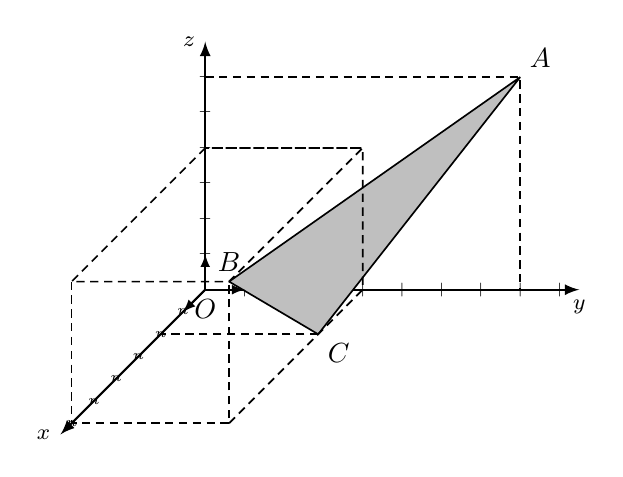
\begin{tikzpicture}[x={(-135:0.4cm)},y={(0:0.5cm)},z={(90:0.45cm)},line join=bevel]
		\coordinate (O) at (0,0,0) ; \draw (O) node[below] {$O$} ;
		\coordinate (A) at (0,8,6) ; \draw (A) node[above right] {$A$} ;
		\coordinate (B) at (6,4,4) ; \draw (B) node[above] {$B$} ;
		\coordinate (C) at (2,4,0) ; \draw (C) node[below right] {$C$} ;
		\draw[thick,->,>=latex] (O)--++(6.5,0,0) node[left,font=\footnotesize] {$x$} ;
		\foreach \x in {1,2,...,6} \draw (\x,0,0) node[font=\tiny] {$\textbackslash$} ;
		\foreach \y in {1,2,...,9} \draw (0,\y,0) node[font=\tiny] {$|$} ;
		\foreach \z in {1,2,...,6} \draw (0,0,\z) node[font=\tiny] {$-$} ;
		\draw[thick,->,>=latex] (O)--++(0,9.5,0) node[below,font=\footnotesize] {$y$} ;
		\draw[thick,->,>=latex] (O)--++(0,0,7) node[left,font=\footnotesize] {$z$} ;
		\draw[semithick,fill=lightgray] (A)--(B)--(C)--cycle ;
		\draw[semithick,densely dashed] (0,0,6)--(A)--(0,8,0) ;
		\draw[semithick,densely dashed] (0,0,4)--(6,0,4)--(B)--(0,4,4)--cycle ;
		\draw[semithick,densely dashed] (6,0,4)--(6,0,0)--(6,4,0)--(B) ;
		\draw[semithick,densely dashed] (6,4,0)--(0,4,0)--(0,4,4)--(0,0,4) ;
		\draw[semithick,densely dashed] (C)--(2,0,0) ;
		\draw[semithick,->,>=latex] (O)--++(1,0,0) ;
		\draw[semithick,->,>=latex] (O)--++(0,1,0) ;
		\draw[semithick,->,>=latex] (O)--++(0,0,1) ;
	\end{tikzpicture}
\end{center}

\begin{enumerate}
	\item 
	\begin{enumerate}
		\item Justifier que les points $A$, $B$ et $C$ ne sont pas alignés.
		\item Montrer que le vecteur $\vect{n}(1;2;-1)$ est un vecteur normal au plan $(ABC)$.
		\item Déterminer une équation cartésienne du plan $(ABC)$.
	\end{enumerate}
	\item Soient $D$ et $E$ les points de coordonnées respectives $(0;0;6)$ et $(6;6;0)$.
	\begin{enumerate}
		\item Déterminer une représentation paramétrique de la droite $(DE)$.
		\item Montrer que le milieu $I$ du segment $[BC]$ appartient à la droite $(DE)$.
	\end{enumerate}
	\item On considère le triangle $ABC$.
	\begin{enumerate}
		\item Déterminer la nature du triangle $ABC$.
		\item Calculer l'aire du triangle $ABC$ en unité d'aire.
		\item Calculer $\vect{AB}  \cdot \vect{AC}$.
		\item En déduire une mesure de l'angle $\widehat{BAC}$ arrondie à $0,1$ degré.
	\end{enumerate}	
	\item On considère le point $H$ de coordonnées $\left(\dfrac53;\dfrac{10}{3};\dfrac53\right)$.
	
	Montrer que $H$ est le projeté orthogonal du point $O$ sur le plan $(ABC)$.
	
	En déduire la distance du point $O$ au plan $(ABC)$.
\end{enumerate}